\chapter{Die Quantitätstheorie}

\section{Geschichte der Quantitätstheorie}
Die Quantitätstheorie hat ihren Ursprung bereits im 16. Jahrhundert. Bereits damals wurde argumentiert, dass der Zufluss an Gold und Silber (aus der neuen Welt) die Preise vorort beeinflusste. Dies Bedeutet also konkret, dass bereits im Mittelalter bekannt war, dass die Menge der Zahlungsmittel die Höhe der Preise bestimmt \autocite{Woll1977}. \\
Dieses Denken wurde dann Anfang des 19. Jahrhundert aus ökonomischer Sicht betrachtet. Im weiteren Verlauf der Entwicklung der Quantitätstheorie nahmen namhafte Ökonomen wie Ives Fisher oder Milton Friedman weitere Versuche der Spezifizierung vor. Friedman ging mit der Theorie sogar soweit, dass er die Finanzkrise in den USA zu beginn der 1930er Jahre damit begründete, dass eine sich verschäfende Geldwertpolitik die Ursache für ebendise Krise war. \\
Die Quantitätstheorie entwickelte sich mit und vor allem als Gegenpol zur nachfrageorientierten Inflationstheorie, welche durch Keynes und der durch ihn begründeten Ideologie des Keynesianismus geprägt wurde.

\section{Allgemeine Quantitätsformel}

Die grundsätzliche Aussage der Quantitätstheorie, die vorhandene Geldmenge beeinflusst die Entwicklung der Preise wurde durch folgende Formel ausgedrückt:
$$ M \cdot V = T \cdot P$$\label{allg. Q-Formel}

Die Formel soll nun analysiert werden und die allgemein bekannte Quantitäts-formel daraus abgeleitet werden. Im ersten Schritt muss verstanden werden, wofür die beiden Seiten der Formel stehen und was diese Bedueten. 
Beginnend mit der linken Seite stellt man fest, dass dort das Produkt der vorhandenen Geldmenge $M$ und der Geldumlaufgeschwindigkeit $V$ betrachtet wird. Mithilfe der Logik ergibt sich, dass dies nichts anderes darstellt, als die "Summe aller Zahlungen" in einem Wirtschaftssystem. Die Umlaufgeschwindigkeit $V$ spielt später bei der Herleitung der allg. Quantitätsformel eine sehr wichtige Rolle. \\
In der Quantitätstheorie wird die Summe der Zahlungen nun dem Produkt aus der Anzahl aller Transaktionen $T$ und dem durchschnittlichen Preis $P$ gegenübergestellt. Auch hier kann nun festgestellt werden, dass dieses Produkt nichts anderes darstellt als die \textbf{Summe des Wertes aller Käufe} in einer Volkswirtschaft. Nun lässt sich allerdings auch argumentieren, dass es sich hierbei um eine Tautologie handelt, da die Summe dessen, was gezahlt wurde immer gleich der Summe des Wertes aller Käufe ist.

Nun stellt sich aber die Frage der Messbarkeit der einzelnen Komponenten dieser Formel. Die Geldmenge lässt sich einfach messen und bestimmen. Bekannte Größen wären z.B. die $M_0$, $M_1$,$M_2$ oder $M_3$. Eine genaue Bestimmung aller anderen Faktoren lässt sich leider nicht verlässlich durchführen, vor allem da immer die Gesamtheit einer Volkswirtschaft betrachtet werden muss. Ein Großteiler aller Transaktionen beispielsweise sind Finanztransaktionen und nicht Interaktionen zwischen einem Enverbraucher und einem Geschft, wie beispielsweise einem Supermarkt. Gleichzeitig ist es quasi unmöglich die genaue Umlaufgeschwindigkeit $V$ der Geldmenge zu bestimmen, zumal diese entsprechend der Wahl der Geldmengengröße auch angepasst werden muss. \\
Ein durchschnittlicher Preis auf Basis der Transaktionen lässt sich mit gleicher Argumentation nicht bestimmten, da zur Berechnung eines Durchschnitts sowohl Anzahl, als auch die Messgröße (hier der Preis einer Transaktion) bekannt sein muss.

Somit stellt diese Formel zwar einen auf Basis der Logik betrachteten Sachverhalt schlüssig dar, ein empirischer Beweis dafür ist allerdings sehr schwer aufzustellen aufgrund der schwierigen Messbarkeit der einzelnen Bestandteile der Formel.

\section{Herleitung der eigentlichen Quantitätsformel}

Im weiteren Entwicklungsverlauf der Theorie wurde versucht die Formel so zu spezifizieren, dass sie zugänglicher wird. Gleichzeitig sollte erreicht werden, dass auch mit Werten gearbeitet werden kann, welche im Rahmen einer Volkswirtschaft bekannt sind.

Die Einschränkung, die diese Spezifizierung ermöglicht, betrifft das Transaktionensvolumen $T$. Anstelle \textbf{aller} Transaktionen werden innerhalb der Formel nur die Transaktionen betrachtet, welche eine Auswirkung auf das BIP $Y$ haben. Dabei fällt also der oben bereits erwähnte größte Anteil der Transaktionen, nämlich die Finanztransaktionen, weg. Das BIP ist eine gut messbare und bekannte Größe innerhalb einer Volkswirtschaft. Allerdings gilt es jetzt, da es sich bei der Gleichung um eine Identität handelt, auch die Gegenseite anzupassen, um sicherzustellen, dass es sich bei der Gleichung um eine wahre Aussage handelt. Die betrachtete Geldmenge ist bereits bekannt und auch Messbar, wie bereits oben festgestellt werden konnte. Also gilt es nun zu versuchen die Umlaufgeschwindigkeit $V$ näher bestimmen zu können. Da auch diese Abhängig von der Anzahl und Art der Transaktion ist wird nun versucht die Umlaufgeschwindigkeit des Geldes auf Basis des BIP zu bestimmten.

Dies führt zu einer neuen Formel: 

$$ M \cdot V_Y = Y \cdot P$$\label{QFormel}
In der Literatur wird die Formel dabei auch ohne den Index bei der Umlaufgeschwindigkeit geschrieben.

$$ M \cdot V = Y \cdot P$$

Dies verleitet einen unerfahrenen Ökonomen oftmals dazu sich nicht klarzumachen, dass es sich hierbei nur um die durchschnittliche Umlaufgeschwindigkeit der Geldmenge, welche \textbf{wirksam auf das BIP} sind, handelt.

Eine weitere Annahme, welche bereits Eingangs angepsrochen wurde, ist, dass es sich bei der Umlaufgeschwindigkeit $V_Y$ um einen (annähernd) konstanten Wert $\overline{V}_Y$ handelt. Die Bedeutung dieser Annahme kann am besten anhand eines Beispiels aufgezeigt werden.

\begin{example}[Konstante Umlaufgeschwindigkeit]
    Man nehme einen Haushalt $H$ mit einer angenommenen Geldmenge $M$ von 10.000\EUR, wovon 1000\EUR\ in Form von liquidem Barvermögen vorliegen. Der Rest des Geldes liegt in Form von Aktien oder ähnlichem vor. Die zu betrachtete Geldmenge sei dabei nur auf das Barvermögen beschränkt. \\
    Nun versucht die Zentralbank eine höhere Geldmenge in Umlauf zu bringen, in dem sie Anleihen von Privathaushalten kauft. Hier offenbart sich bereits eine weitere argumentative Lücker innerhalb der Quantitätstheorie. Diese beschreibt nicht, wie eine Erhöhung oder Senkung der Geldmenge beim Endverbraucher ankommt. Von (Friedman/Fisher) kam die Anekdote, dass es sich vorzustellen gilt, dass das Geld aus einem Helikopter abgeworfen wird und von den Verbauchern aufgesammelt wird. Man nehme nun, zum Zweck des Beispiels an, das die Geldmenge würde sich um das aufgekaufte Mass der Zentralbank erhöhen. Somit beläuft sich die Höhe des Barvermögens bei einem Anleihenankauf von 1000\EUR\, des durchschnittlichen Haushalt auf 2000\EUR. 

    Da von einer Konstanz in der Umlaufgeschwindigkeit ausgegangen wird, würde das bedeuten, dass der Endverbraucher bei einer Erhöhung des ihm zur Verfügung stehenden Barvermögens dieses genauso verwendet, wie zuvor. 
\end{example}\label{Bsp.kUmlauf}

Nun stellt sich die Frage, wie diese Formel nun auf Basis der Geldmenge die Veränderung des Preises anzeigen will. Mit der Annahme einer konstanten Umlaufgeschwindigkeit bleiben, um die Identität der Gleichung der wahren, zwei Mögichkeiten:

\subsubsection*{1. Erhöhung der Geldmenge führt zu einer Erhöhung des BIP $Y$ zur Wahrung der Identität:}
Bei dieser Möglichkeit wird davon ausgegangen, dass sich das BIP erhöht, um den Anstieg der Geldmenge auszugleichen. Hierbei gibt es zwei große Probleme:

\begin{enumerate}
    \item Betrachtet man wieder das Beispiel\, \vref*{Bsp.kUmlauf} verdoppelt sich die Geldmenge. Das würde bedeuten, dass sich das BIP ebenfalls verdoppeln müsste, um die Gleichung weiterhin zu erfüllen. Obwohl die Annahme, dass das BIP eine Konstante ist falsch ist, belaufen sich die Schwankungen doch eher auf 2-3\%, nicht, wie in diesem Fall, auf 200\%.
    \item Um das BIP zu erhöhen müsste die erhöhte Geldmenge in Transaktionen verwendet werden, welche wirksam im Bezug auf das BIP sind. Wie bereits zuvor erwähnt ist ein Großteil der Transaktionen innerhalb einer Volkswirtschaft nicht wirk auf das BIP.
\end{enumerate}

Diese Probleme führen zu der Annahme, dass das BIP in der Quantitätstheorie als annähernd konstant interpretiert wird. Somit wird ein kausaler Zusammenhang zwischen der Geldmenge $M$ und er BIP $Y$ ausgeschlossen.

\subsubsection*{2. Erhöhung der Geldmenge führt zu einer Erhähung des Preises $P$}
Diese Möglichkeit würde den eigentlichen Zweck der Theorie erfüllen, da davon ausgegangen wird, dass die Geldmenge der ausschlaggebende Faktor ist, für die Darstellung des Preises.

Laut der Gleichung\, \vref*{QFormel} bedeutet das also, dass ein proportinaler Zusammenhang zwischen der Geldmenge $M$ und dem Preis $P$ besteht, da $\overline{V}_Y$ und $Y$ als annähernd konstant angenommen werden.

Dies führt zu der finalen Spezifizierung, die die Quantitätsformel von der allg. Quantitätstheorie und der darin beschriebenen Identität unterscheidet. Es besteht ein kausaler Zusammenhang zwischen der Geldmenge $M$ und dem durchschnittlichen Preis $P$.
Inhärent hat dies zur Folge, dass durch die Steuerung der Geldmenge auch der \enquote{Wert des Geldes}, also die aktuelle Inflation oder Deflation, gesteuert werden können.

\section{Kritik an der Quantitätstheorie und -formel}

Die Kritik an der Quantitätstheorie ergibt sich aus einem sehr realen Beispiel aus der Ökonomie in Amerika während der Finanzkrise 08/09. Dort argumentiert der Ökonom Paul Krugman folgendermaßen:

\enquote{
[T]he past three years — the post-Lehman era during which the Fed presided over a tripling of the monetary base — have been an excellent test of that model [die Quantitätstheorie], which has failed with flying colors ... [W]hen you triple the monetary base, the resulting inflation shouldn’t be something that depends on the fine details — unless the model is completely wrong.

And the model is completely wrong. You don’t get more conclusive tests than this in economics. [...] 
And this in turn tells you something about the people pushing this stuff. They had a model; it made predictions; the predictions were utterly, totally wrong; and they have just dug in further.
}\autocite{Krugman2011} 

Dieses Zitat bezieht sich, wie bereits oben erwähnt, auf die Finanzkrise und die Art und Weise, wie die FED versucht hat dieser entgegenzuwirken. Nun kommt die Frage auf: Wieso wird genau diese Krise gewählt, um eine Kritik an der Quantitätstheorie zu formulieren. Diese Antwort wird bereits von Krugman in seinem Zitat gebeben:
\begin{center}
    \enquote{You don’t get more conclusive tests than this in economics.}
\end{center}

Es gibt also innerhalb der Ökonomie keine besseren Tests, ob eine Theorie valide ist, oder Schwächen aufweist, als ein Beispiel aus der Realtiät. In folgender Grafik ist zu erkennen, wie sich bei steigender Geldmenge der durchschnittliche Preis in dieser Zeit enwtickelt hat.

\begin{figure}[h]
    \centering
    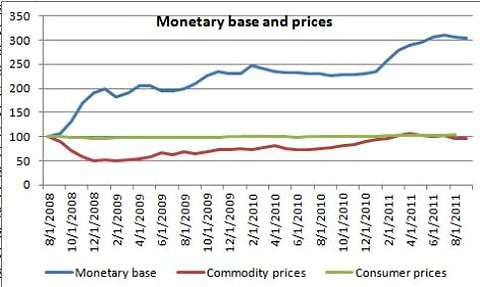
\includegraphics{img/100711krugman3-blog480.jpg}
    \caption{Entwicklung des Preises auf Basis der Geldmenge während der Finazkrise 08/09\autocite*{Krugman2011}}
\end{figure}    

\begin{itemize}
    \item Konstante Umlaufgeschwindigkeit [x]
    \item Wie kommt das geld zum Endverbraucher?
\end{itemize}

\clearpage